\documentclass[11pt,a4paper,twoside]{article}
\usepackage{a4wide}	% für gut definierte Seitenränder und Platzausnutzung
\usepackage[utf8]{inputenc}	% für Umlaute
\usepackage{amssymb,amsmath}
\usepackage{booktabs}   % schöne Tabellen
\usepackage[pdftex]{graphicx}
\graphicspath{{./pic/}}
\usepackage{epstopdf}
\usepackage{siunitx}	% für SI-Einheiten; siehe http://mirror.unicorncloud.org/CTAN/macros/latex/contrib/siunitx/siunitx.pdf
\usepackage[version=3]{mhchem}	% chemische Symbole mit \ce{}
\usepackage{listings} 	% für Einbinden von Quellcode
\usepackage{color}	% für das Einfärben von eingebundenem Quellcode
\usepackage{longtable}	% für das Erstellen mehrseitiger Tabellen
\usepackage[german]{isodate} % Datumformatierung für \today
\usepackage{marvosym}
\usepackage{ulem}	% 

% declaring custom units
\DeclareSIUnit \mag {mag}
\DeclareSIUnit \parsec {pc}
\DeclareSIUnit \AU {AU}
\DeclareSIUnit \pixel {pixel}

% format angle display
\sisetup{add-arc-degree-zero}
\sisetup{add-arc-minute-zero}
\sisetup{add-arc-second-zero}
\sisetup{arc-separator = \,}


%Befehl, um Quellcode einzufügen: 
%\lstinputlisting[caption = {``title``}, captionpos = b, language=C++]{data.cpp}

%Befehl, um Graphik einzufügen:   
%\begin{figure}
%  \centering
%  \includegraphics[width=0.7\textwidth, angle=-90]{center_diff.eps}
%  \caption{centered differencing at t = 4}
%\end{figure}

% Befehl für kein ``\noindent mehr''
\setlength\parindent{0pt}

%\lstset{numbers=left}

\newcommand{\op}[1]{\operatorname{#1}}

% Konsistente Variablennamen:
\newcommand{\zen}{\ensuremath{\nu} }    % zenith angle
\newcommand{\hei}{\ensuremath{h} }      % height angle
\newcommand{\HA}{\ensuremath{\Gamma} }  % hour angle \HA
\newcommand{\DEC}{\ensuremath{\delta} } % declination \DE
\newcommand{\LAT}{\ensuremath{\Phi} }   % latitude \LAT
\newcommand{\electron}{\ce{e^-}}
\newcommand{\SNR}{\ensuremath{\frac{S}{N}} }

\newcommand{\MgFe}{\ensuremath{[\text{MgFe}]^\prime} }
\newcommand{\ZH}{\ensuremath{[\text{Z}/\text{H}]} }
\newcommand{\Hbo}{\ensuremath{[\text{H}\beta_0]} }

\lstset{
   basicstyle=\scriptsize\ttfamily,			% grundlege des Design
   keywordstyle=\ttfamily,				% Design von Schlüsselwörtern (Codebefehle wie Variablentypen, Schleifenbefehle u.Ä.)
   stringstyle=\ttfamily,				% Design von Variablen
   commentstyle=\ttfamily\color{blue},			% Design von Kommentaren
   showstringspaces=false,				% Leerzeichen in Strings darstellen?
   flexiblecolumns=false,				% dynamische Spaltenbreite?
   tabsize=2,						% Länge des Tabulators
   % Einstellung der Zeilennummerierung:
   numbers=left,					% Position der Nummern
   numberstyle=\tiny,					% Größe der Nummern
   numberblanklines=true,				% Leerzeilen durchnummerieren?
   numbersep=20pt,					% Platz zwischen Nummern und Code
   xleftmargin=30pt					% Platz zum linken Seitenrand
 }
 
%opening
\title{\LARGE \underline {Sheet 5}}
\author{Johannes Haux \\ Florian Trost \\ Elsa Wilken}
\date{\today}


\begin{document}

\maketitle
\thispagestyle{empty}

\begin{center}
  Astronomical Techniques (MKEP5) \\
  \baselineskip35pt
  by Prof. Dr. Stefan Wagner and Priv.-Doz. Dr. Thorsten Lisker \\
  \baselineskip60pt
  Ruprecht Karl University of Heidelberg
\vskip 40pt

\includegraphics[width=5cm]{UniHD.png}

\end{center}

\newpage
\setcounter{page}{1}		% set page count to start with 1 here

\section*{Exercise A.}

\section*{Exercise B.}

According to the virial theorem, galaxies in an isolated cluster can change
their kinetic ($K$) and potential energies ($W$) as long as the sum of these 
remains constant, so that $K = -0.5W$. Here, $W$ is the potential energy of the 
galaxies within the gravitational potential of the cluster, $W \propto 
G \frac{M_{clu}}{R_{clu}}$, where $M_{clu}$ and $R_{clu}$ are the total mass and 
the radius of the cluster, and $G$ the gravitational constant. We have to keep 
in mind that cluster galaxies move because of the Universe expansion and 
because of their orbits in the cluster potential well. \\

\paragraph{1.} By applying the virial theorem, astronomers were able to 
estimate the total mass of the Abell 1689 cluster (see Fig. 1 on sheet) and of 
other galaxy clusters. Which kind of observations would you need to compute 
the total mass of a cluster? (6 points) \\

As we know $W$ and $K$ are defined as follows:
\begin{align}
    W   &= \sum_i W_i \\
        &= \sum_i - \int_{\infty}^{R_{clu}} \vec{F}_i(\vec{r})\op{d}\vec{r} \\
        &= \sum_i - \int_{\infty}^{R_{clu}} -\frac{GM_{clu}m_i}{r^2}\op{d}r \\
        &= \sum_i GM_{clu}m_i\int_{\infty}^{R_{clu}} \frac{1}{r^2}\op{d}r \\
        &= -\left( \sum_im_i \right)GM_{clu} \frac{1}{R_{clu}}  \\
        &= \frac{GM_{clu}^2}{R_{clu}}
\end{align}
Here we assume, that $M_{clu} \gg m_i$ and a spherical distibution.
The total potential energy is the sum of all the potential energies each 
member of the cluster has.
\begin{align}
    K   &= \sum_i \frac{1}{2}m_iv_i^2\;,\\
        &= \frac{1}{2} M_{clu} \left< v^2\right> \;, \\
        &= \frac{3}{2} M_{clu} \sigma^2\;,
\end{align}
with $m_i$ and $v_i$ being the masses and velocities of the members of the
cluster, which sum up to total mass $M_{clu}$ and the mean-squared velocity
$\left< v^2 \right>$, which in turn can be described via the measured radial
velocity dispersion $\sigma$. Also, from the deep and never ending ocean of
information, that we call the internet, we know that 
$3\sigma^2 = \left<v^2\right>$.

Now we can use virial's theorem to find a descripton of $M_{clu}$, dependend
only on observable magnitudes:
\begin{align}
    -0.5\cdot G \frac{M_{clu}^2}{R_{clu}} &\propto \frac{3}{2} M_{clu} \sigma^2\\
    \Leftrightarrow const &= M_{clu} \cdot\left( \frac{1}{3}\frac{G}{\sigma^2 R_{clu}}\right) \\
    \Leftrightarrow M_{clu} &= const \cdot \sigma^2 R_{clu}
\end{align}
In the last step we move all the constants together into $const$, such that we
are only left with the two observables $\sigma^2$, the radial velocity dispersion
and $R_{clu}$, the radius of the cluster, which we both need
to measure to estimate the mass of the cluster.

\paragraph{2.} We can use the spectroscopic information collected for the 
early-type galaxies in this cluster to estimate the age and metallicity of 
their stellar populations (see Fig. 2 on sheet). This is typically done by comparing 
the measured equivalent widths of the index $\Hbo$ and the composite index 
$\MgFe$ with their theoretical values as derived from synthetic simple
stellar populations of given age, metallicity and IMF.\\

Using the attached file \verb+theory_indices.dat+, which list the theoretical 
values of $\Hbo$ and $\MgFe$, draw the grid of theoretical indices as 
displayed in Fig. 3 on the sheet, where the horizontal blue lines show how 
these indices vary as a function of metallicity $\ZH$ (from 
\SIrange{-0.16}{0.16}{dex}) at fixed age, and the vertical red lines show how 
the two indices vary as a function of age (from \SIrange{4}{14}{Gyr}) 
at fixed metallicity $\ZH$. Subsequently, overplot on the theoretical grid 
the observed values of $\Hbo$ and $\MgFe$ that are included in the attached 
file \verb+observed_indices.dat+. By comparing the positions of the observed 
indices with the theoretical grid, estimate the age and metallicity $\ZH$ of 
a sample of early-type galaxies in Abell 1689. Briefly comments your results. 
(8 points) \\

\begin{figure}[h!]
\centering
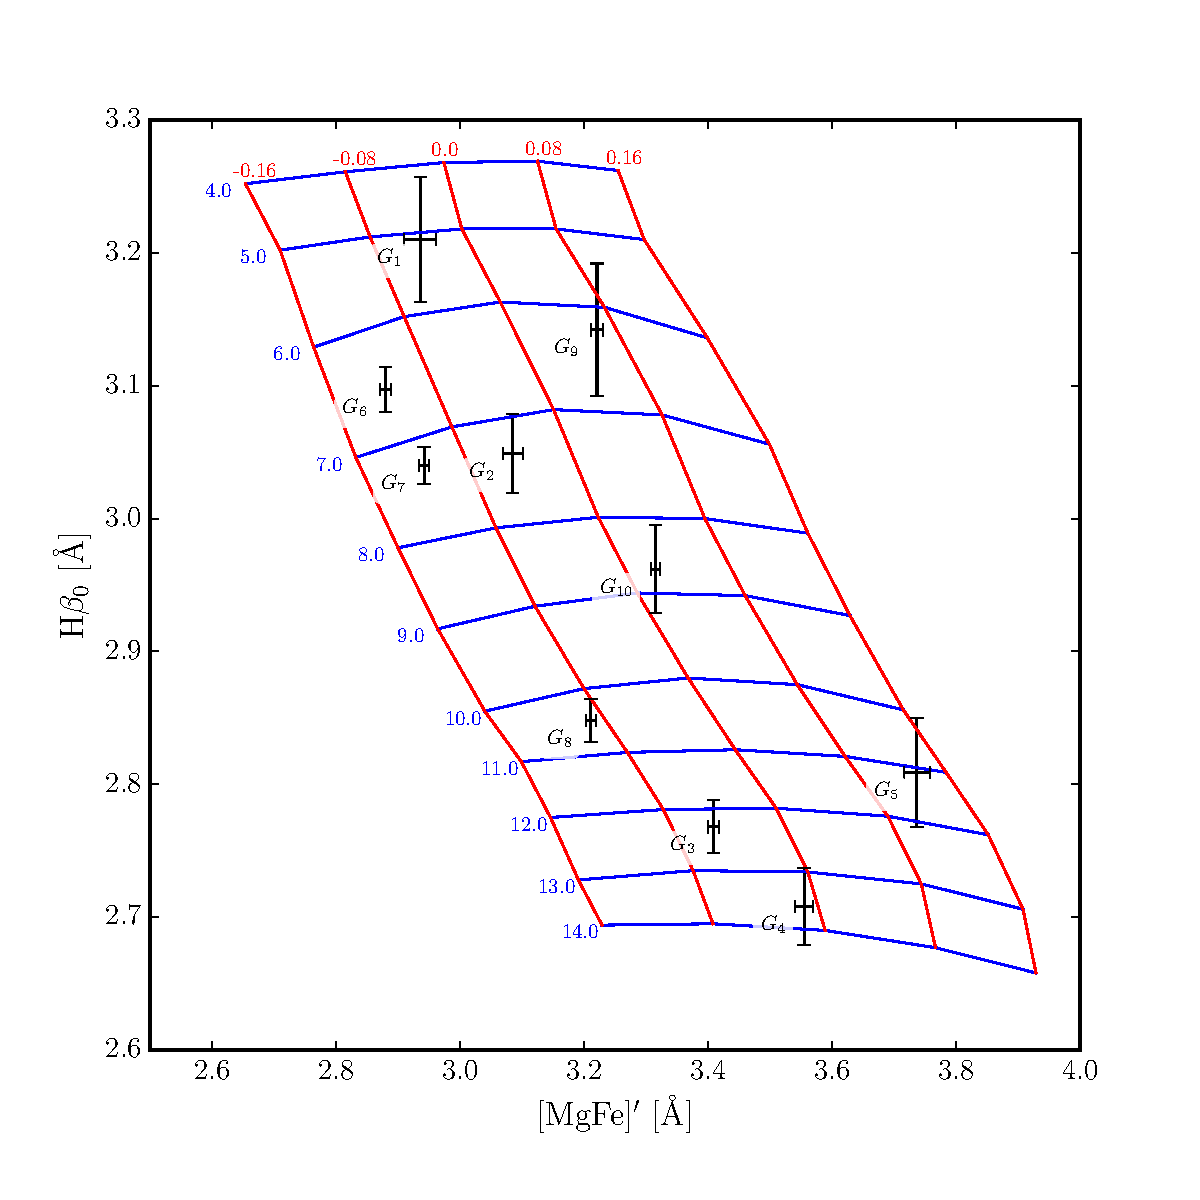
\includegraphics[width=12cm]{ageMetal}
\caption{Measured \MgFe and \Hbo indeces together with model predictions
for age and metalicity.}
\label{fig:am}
\end{figure}
In figure \ref{fig:am} we plot the model and observed data as given in the
exercise. By interpolating linearly by hand we calculate the ages and
metalicities given in table \ref{tab:am}.  

We can see galaxies formed at very early ages of the universe and galaxies,
formed recently. There does not seem to be a correlation between age and 
metalicity.

\begin{table}[h!]
\centering
\begin{tabular}{ccc}\toprule
Galaxy  & \ZH           & age               \\
        & $[\si{dex}]$  & $[\si{Gyr}]$      \\ \midrule
$G_1$   & -0.04         & 5.1				\\
$G_2$   & -0.04	        & 7.4				\\
$G_3$   & -0.05	        & 12.3				\\
$G_4$   & -0.01	        & 13.7				\\
$G_5$   & 0.13	        & 11.1				\\
$G_6$   & -0.12	        & 6.5				\\
$G_7$   & -0.11	        & 7.3				\\
$G_8$   & -0.09	        & 10.5				\\
$G_9$   & 0.07	        & 6.3				\\
$G_{10}$& 0.02	        & 8.6				\\
\bottomrule
\end{tabular}
\caption{Estimated metalicities and ages for the given data in
exercise B. All estimations are done by hand and in a linear 
fashion.}
\label{tab:am}
\end{table}


\section*{Exercise C.}

\paragraph{1.} Which kind of observations would you design in order to measure
the total luminosity in $\text{H}\alpha$ of a HII region? (2 points) \\


\paragraph{2.} The oxygen emission lines in the spectrum of a HII region are
used to measure the abundance of oxygen $ \left[12 + \log{\left( \text{O/H}
\right)} \right]$ in the interstellar medium of a galaxy. Often, the oxygen
abundances of HII regions are plotted as a function of distance from the galaxy
centre so to derive the radial gradient of O/H. Using the data in the attached
file \verb+h2regions.dat+ estimate the radial gradient of O/H for the Milky
Way. Briefly discuss your results. (4 points) \\

In Figure \ref{fig:oxygen} the oxygen abundance given for \num{26} HII regions
in the Milky Way are plotted as a function of their given distance from the
galactic centre. In the upper plot, the given values of oxygen abundance $
\left[12 + \log{\left( \text{O/H} \right)} \right]$ in dex were directly used;
the lower plot shows a linearised variant of the oxygen abundance which was
computed by using the given values subtracted by \num{12} as the exponent of
\num{10}. \\

\begin{figure}[h!]
\centering
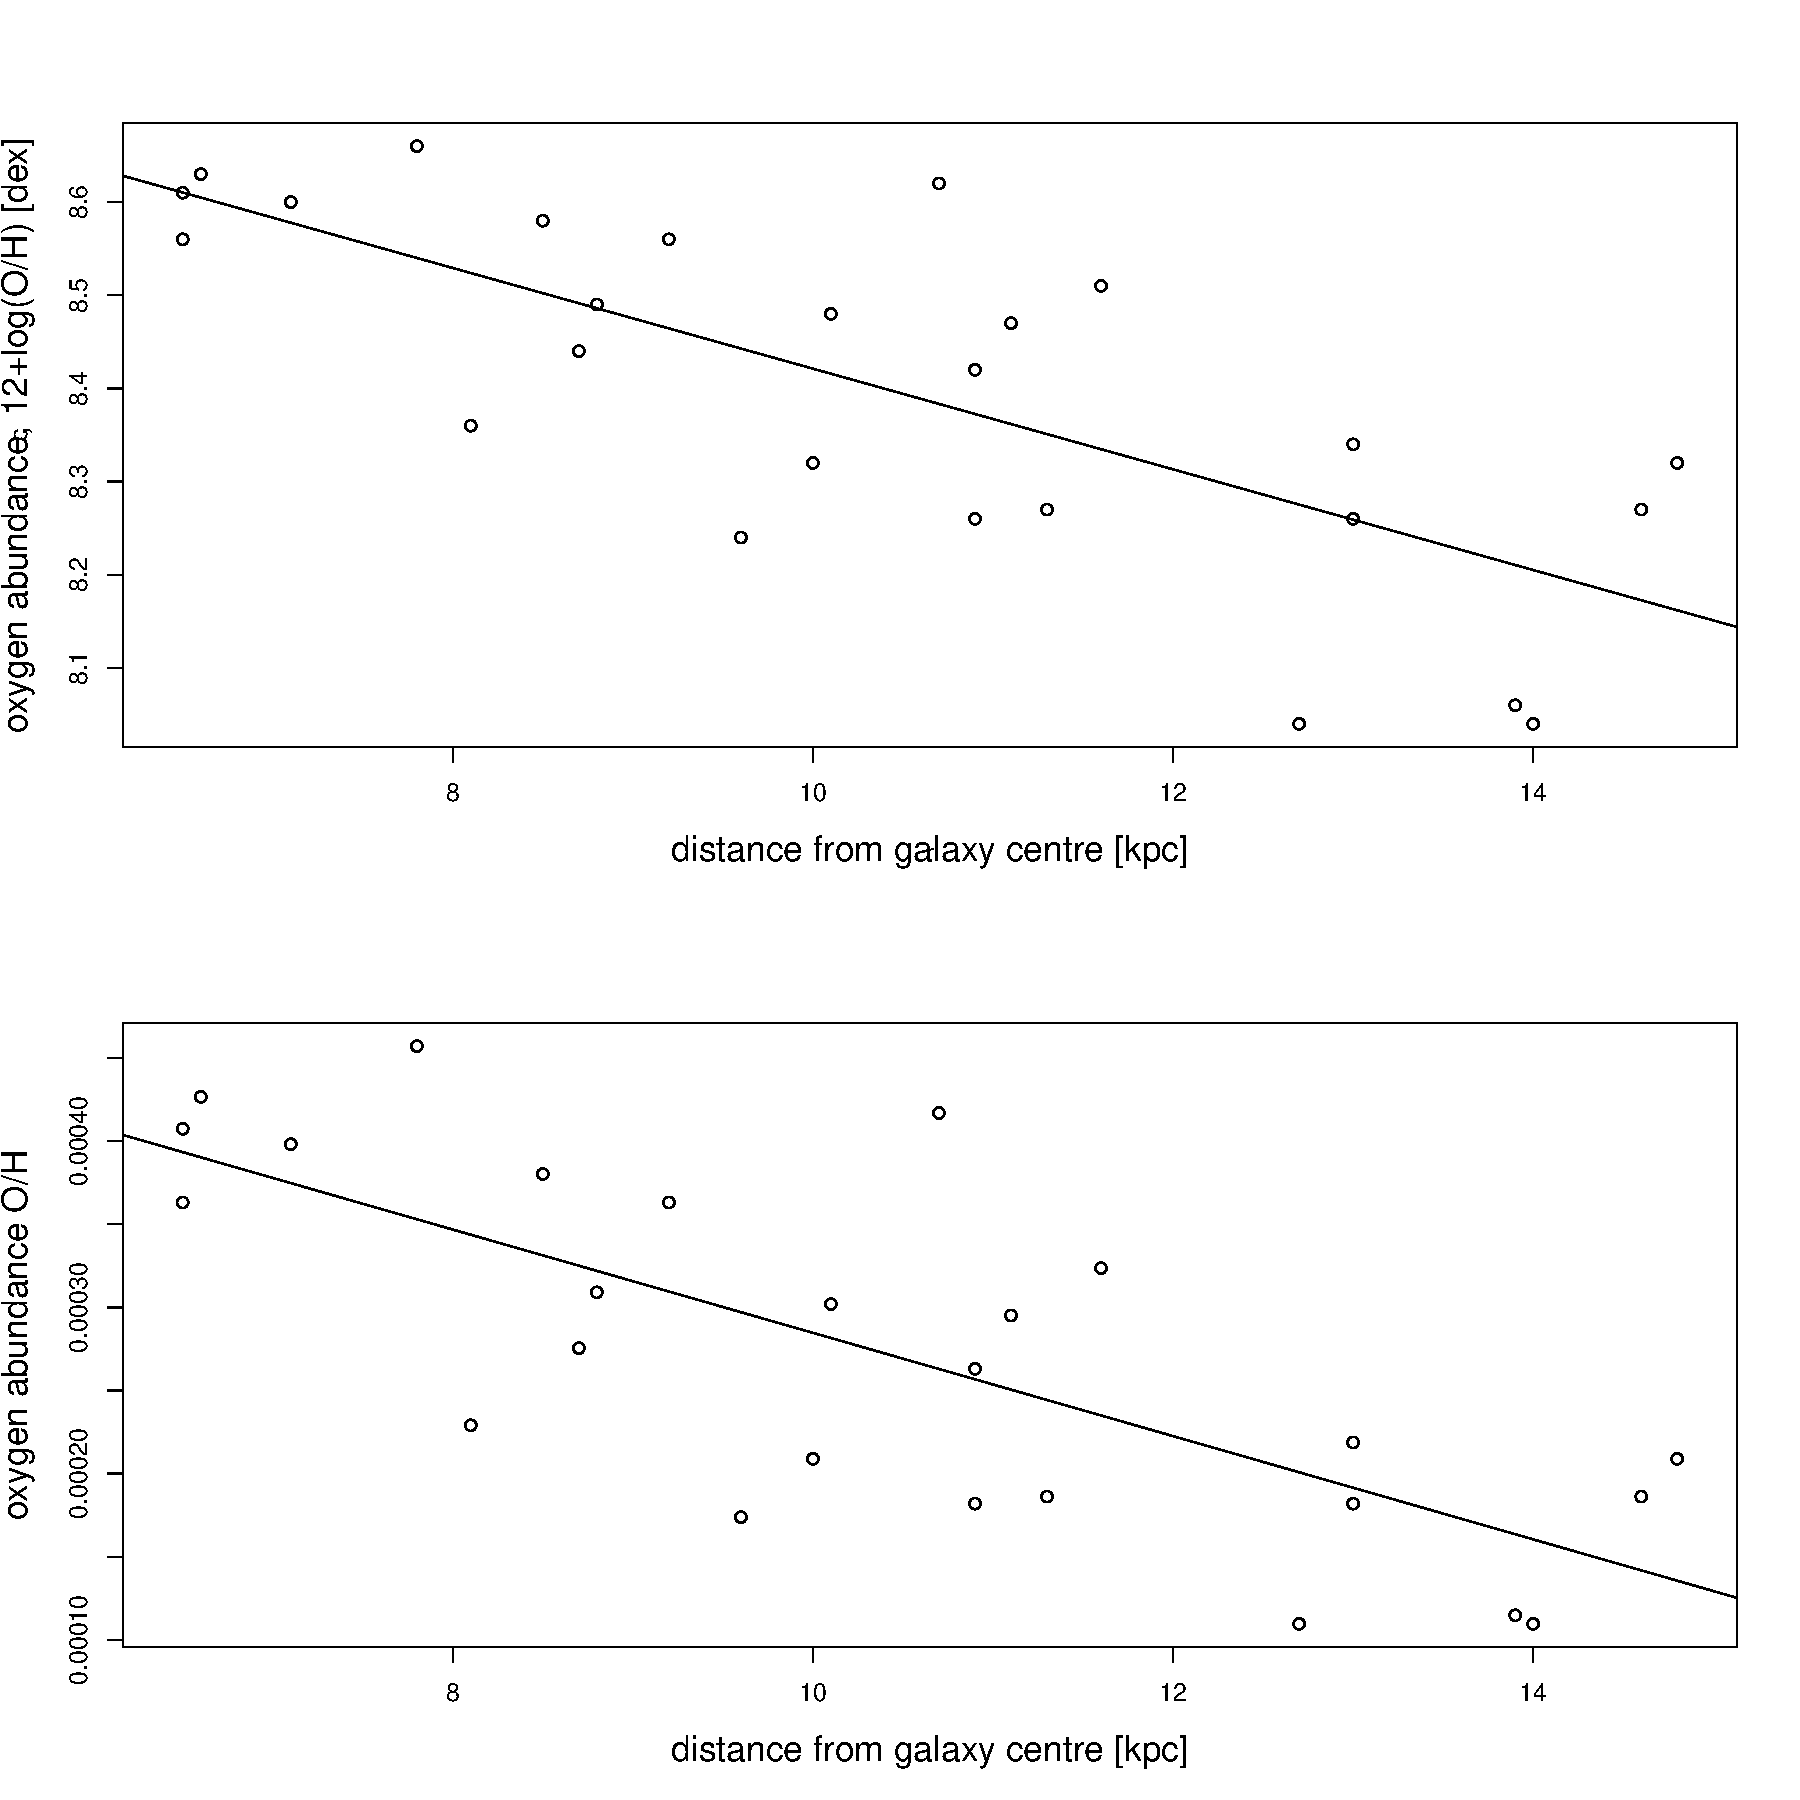
\includegraphics[width=\textwidth]{oxygen}
\caption{Oxygen abundance for different HII regions in the Milky Way as a
function of distance from galaxy centre; top: oxygen abundance $ \left[12 +
\log{\left( \text{O/H} \right)} \right]$ in dex; bottom: oxygen abundance O/H;
the straight lines are models computed via simple linear regression.}
\label{fig:oxygen}
\end{figure}

For each case, a simple linear regression was computed. The coefficients of the linear models are listed in Table \ref{tab:oxygen}. 

\begin{table}[h!]
\centering
\begin{tabular}{lcc}\toprule
		  & Intercept		& Slope			\\ \midrule
original data	  & \num{8.96}		& \num{-0.054}		\\
linearised data   & \num{5.95e-4}	& \num{-3.105e-5}	\\
\bottomrule
\end{tabular}
\caption{Coefficients of the linear models for both original and linearised data.}
\label{tab:oxygen}
\end{table}

In the plots of the data a clear trend of decreasing oxygen abundance with
increasing distance from the galactic centre can be seen. This trens is
supported by the linear models which both show a negative slope. According to
the linear models, the oxygen abundance decreases with \num{-0.054} dex per
kiloparsec. The overall trend of lower oxygen abundance in the outer regions of
the galaxy indicates a generally lower metallicity in these regions. This is
plausible because star formation rates have been higher in the denser centre of
the galaxy. This led to higher formation rates of heavy elements by
nucleosynthesis in those stars compared to the outer regions of the galaxy. \\

\end{document}
